\documentclass{beamer}
\usepackage{graphicx}
\usepackage[utf8]{inputenc}
\usepackage{amsmath}
\usepackage{graphics}
\usepackage{xcolor}
\usepackage{listings}
\usepackage{adjustbox}
\lstnewenvironment{rcode}{
	\lstset{language=R,
		basicstyle=\small\ttfamily,
		commentstyle=\color{gray},
		keywordstyle=\color{blue},
		stringstyle=\color{red},
		showstringspaces=false,
		breaklines=true,
		frame=single,
		captionpos=b,
		numbers=left,
		numberstyle=\tiny\color{gray},
		stepnumber=1,
		numbersep=5pt
	}
}{}

\usepackage{tikz}
\usepackage{wasysym}
\usetikzlibrary{calc,shapes, arrows, positioning, shapes.gates.ee, trees}
\usepackage{hyperref}
\usepackage{booktabs}
\usepackage{multirow}
\title{METHODOLOGY}
\author{KENNEDY, CHARLES, BEVERLY, DOKTA AND DOMINIC}
\begin{document}
	\maketitle
	\begin{frame}{Introduction}
		In this chapter, we discuss the CFA model, Invariance measurement, research approach, the procedures used to obtain the data, methods used to analyze the data and the models used.
	\end{frame}
\begin{frame}{Conceptual Introduction to Confirmatory Factor Analysis}
	
	Confirmatory factor analysis (CFA) is a type of structural equation (SEM) that deals specifically with measurement models, that is, the relationship between observed measures or indicators (e.g test items, test scores, behavioral observation ratings) and latent variable or factor. CFA, unlike its counterpart, exploratory factor analysis, all its aspects must be pre-specified. Therefore, it is required that the researcher has a firm prior idea, based on the pre-existing evidence and theory, of
	number of factors in the data. In CFA, instead of letting the data tell us the factor structure, we pre-determine the factor structure and verify the psychometric structure of previously developed scale. CFA became more popular after a breakthrough in both computing technology on an estimation method developed by Joreskog (1969) ((Brown and Moore, 2012).
\end{frame}
\begin{frame}{Characteristics of CFA Model}
	\begin{enumerate}
		\item Each indicator is continuous with two causes—a single factor that the indicator is supposed to measure and all unique sources of influence represented by the error term.
		\item The error terms are independent of each other and of the factors.
		\item All associations are linear and the factors covary. This is why the symbol for an unanalyzed association in \ref{fig:Figure 3.1} is depicted as solid instead of dashed.
	\end{enumerate}
\end{frame}
\begin{frame}{Advantages of CFA}
	\begin{enumerate}
		\item CFA unlike EFA allows for the specification of relationships among the indicator uniqueness (error variances), which may have substantive importance (e.g. correlated errors due to method effects)
		\item CFA offers a very strong analytic framework for evaluating the equivalence of measurement models across distinct groups. This is accomplished by multiple group solutions or MIMIC models.
		\item CFA has the ability to estimate the relationships among variables adjusting for measurement error
	\end{enumerate}
\end{frame}
\begin{frame}{Advantages of CFA}
	\begin{enumerate}
		\item CFA unlike EFA allows for the specification of relationships among the indicator uniqueness (error variances), which may have substantive importance (e.g. correlated errors due to method effects)
		\item CFA offers a very strong analytic framework for evaluating the equivalence of measurement models across distinct groups. This is accomplished by multiple group solutions or MIMIC models.
		\item CFA has the ability to estimate the relationships among variables adjusting for measurement error
	\end{enumerate}
\end{frame}
\begin{frame}{Assumptions of CFA models}
	\begin{enumerate}
		\item Multivariate normality (i.e the univariate distributions and the joint distribution of all variable combinations are normal)(Kline,2006)\\
		\textbf{\underline{Note}}\\
		Violations of this assumption can lead to a distortion of goodness fit model related to the model as a whole.
		\item sufficient sample size($\geq$ 200)
		\item Correct a priori model specification
		\item Data must come from a random sample
	\end{enumerate}
\end{frame}
\begin{frame}{The Confirmatory Factor Analysis Models}{The single factor analysis model}
	This focus on model identification and model fit. The single item factor analysis model is defined as
	\begin{equation}
		y_1=\tau_1 +\lambda_1 \eta + \epsilon_1
	\end{equation}
which is essentially a linear regrestion model with main predictor he factor, being latent or unobserved. $\tau$ is the intercept of the first item, $\lambda_1$ is the factor loading also termed as regression weight of the factor of the first item. $\epsilon_1$ is the residual(error) for the first item.\\
\end{frame}
\begin{frame}
	For a k common factor(s) the CFA model is;\\
	\[
	\left(
	\begin{matrix}
		y_1= \lambda_{11}\eta_1 +...+\lambda_{1k}\eta_k +\epsilon_1 \\
		y_2= \lambda_{21}\eta_1 +...+\lambda_{2k}\eta_k +\epsilon_2 \\
		y_3 = \lambda_{31}\eta_1+...+\lambda_{3k}\eta_k +\epsilon_3 \\
		.                  .              .      \\
		.                  .               .     \\
		.                  .              .     \\
		y_p=\lambda_{p1}\tau_1+...+\lambda_{pk}\tau_k +\epsilon_p \\                
		
	\end{matrix}
	\right)
	\]\\
\end{frame}
\begin{frame}
Which in matrix notation that the form(Johnson,2007 \& UCLA,)\\

\begin{equation}
	\left(
	\begin{matrix}
		y_1\\
		y_2\\
		\vdots \\
		y_p\\
	\end{matrix}
	\right) = 
	\left(\begin{matrix}
		\lambda_{11}\eta_1 & .&.&.& \lambda_{1k}\\
		\lambda_{21}\eta_1 &  .&.&. & \lambda_{2k}\\
		\vdots\\
		\lambda_{p1}\eta_1  & .&.&. &\lambda_{pk}\\
	\end{matrix}\right) \times
	\left(\begin{matrix}
		\eta_1\\
		\eta_2\\
		\vdots\\
		\eta_k\\
	\end{matrix}\right)+ \left(\begin{matrix}
		\epsilon_1\\
		\epsilon_2\\
		\vdots\\
		\epsilon_p\\
	\end{matrix}\right)
\end{equation}\\
\end{frame}
\begin{frame}
	\begin{equation}
		Y=\Lambda\eta_i + \epsilon_i
	\end{equation}
	Where;
	\begin{enumerate}
		
		\item Y- is p $\times$1 vector of the observable random variables
		\item $\Lambda$ is the matrix factor loading
		\item $\eta_i$ refers to the k$\times$1 of the latent(unobservable) variables.
		\item $\epsilon_i$ is a p$\times$1 vector of the residual(errors)
	\end{enumerate}
The equation(3) above looks like a multiple regression model of Y on $\eta$ but it's not testable since the factors $\eta_i$ are unobserved. This model implies a particular form of variance-covariance matrix $\sum$ which is testable.
\end{frame}
\begin{frame}{Two-Factor CFA model}
	Results from the one-factor CFA suggest that a one solution may capture much variance in the observed variables, however the model fit suggests that this model can be improved(Kline,2006).
	Two factor CFA model assumes;
	\begin{enumerate}
		\item Factors are uncorrelated.
		\item Factors are correlated.
	\end{enumerate}
\end{frame}
\begin{frame}{Uncorrelated factors}
Proceeding with a two-factor CFA, we assume uncorrelated (or orthogonal) factors. Having a two-item factor presents a special problem for identification. In order to identify a two-item factor there are two options:
\begin{enumerate}
	\item  Freely estimate the loadings of the two items on the same factor but equate them to be equal while setting the variance of the factor at 1.
	\item Freely estimate the variance of the factor, using the marker method for the first item, but covary (correlate) the two-item factor with another factor.
\end{enumerate}
\end{frame}
\begin{frame}{Correlated factors}
We still have the issue of that two-item factor.in model identification we can either equate the loadings and set the variance to 1 or we can covary the two-item factor with another factor and use the marker method(Brown,1960)
\end{frame}
\begin{frame}{The General CFA Model}
	All models in the CFA contain factor variance, unique variance and factor loadings.\\
	\textbf{The factor loadings} are the regression slopes for predicting the latent factor.\\
	\textbf{The factor variance} expresses sample variability or dispersion of the factor, that is, the extent to which sample participants\\ relative standing on the latent dimension is similar or different. 
	\textbf{Unique variance or error variance} is typically the unwxplained variation or simply the measurement error.\\
	As an illustration we can represent CFA model as shown in the \ref{fig:Figure 3.1} below;
\end{frame}
\begin{frame}
\begin{figure}
	\centering
	\begin{adjustbox}{max width=\textwidth}
		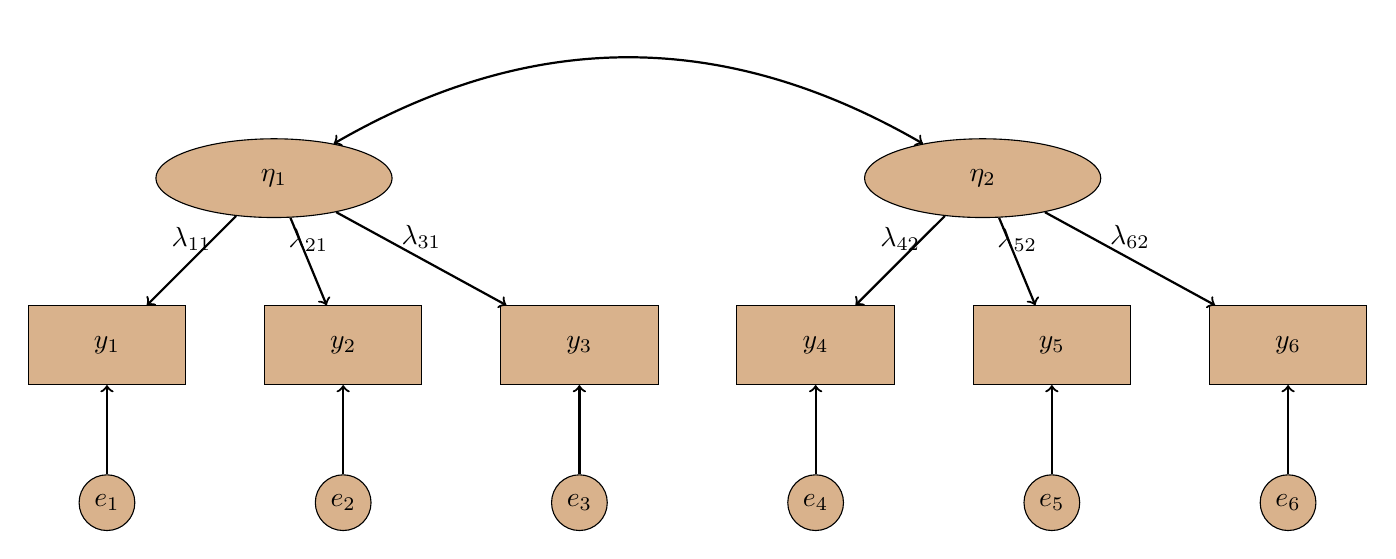
\begin{tikzpicture}[ factor/.style={draw,fill=brown!60, ellipse,minimum height=1cm, minimum width=3cm, node distance= {9cm}},
			latent/.style={draw,fill=brown!60, rectangle, minimum width=2cm, minimum height=1cm, node distance= {3cm}},
			residual/.style={draw,fill=brown!60,  circle, node distance= {2cm}}
			]
			\node [factor](x1) {$\eta_1$};
			\node [factor](x2)[right of =x1] {$\eta_2$};
			\node [latent](y1) [below left of=x1] {$y_1$};
			\node [latent](y2) [right of=y1] {$y_2$};
			\node [latent](y3) [right of=y2] {$y_3$};
			\node [latent](y4) [right of =y3] {$y_4$};
			\node [latent](y5) [right of=y4] {$y_5$};
			\node [latent](y6) [right of=y5] {$y_6$};
			\node [residual](e1) [below of=y1] {$e_1$};
			\node [residual](e2) [below of=y2] {$e_2$};
			\node [residual](e3) [below of=y3] {$e_3$};
			\node [residual](e4) [below of=y4] {$e_4$};
			\node [residual](e5) [below of=y5] {$e_5$};
			\node [residual](e6) [below of=y6] {$e_6$};
			
			\draw[thick, black, ->](x1) -- (y1) node[midway, above] {$\lambda_{11}$};
			\draw[thick, black, ->] (x1) -- (y2) node[midway, above] {$\lambda_{21}$};
			\draw[thick, black, ->] (x1) -- (y3) node[midway, above] {$\lambda_{31}$};
			\draw[thick, black, ->] (x2) -- (y4) node[midway, above] {$\lambda_{42}$};
			\draw[thick, black, ->] (x2) -- (y5) node[midway, above] {$\lambda_{52}$};
			\draw[thick, black, ->] (x2) -- (y6) node[midway, above] {$\lambda_{62}$};
			\draw[thick, black, ->] (e1) -- (y1);
			\draw[thick, black, ->] (e2) -- (y2);
			\draw[thick, black, ->] (e3) -- (y3);
			\draw[thick, black, ->] (e4) -- (y4);
			\draw[thick, black, ->] (e5) -- (y5);
			\draw[thick, black, ->] (e6) -- (y6);
			\draw[thick, black, <->] (x1) edge[bend left=30] node[above] {} (x2);
		\end{tikzpicture}
	\end{adjustbox}
	\caption{Two factor CFA model with no error covariance}
\label{fig:Figure 3.1}
\end{figure}
\end{frame}
\begin{frame}
Where $\lambda_i$ is factor loading; $e_i$ (for i= 1,.., 6) is the error variance. The covariate line $\eta_1$.$\eta_2$ is the factor variance covariance.\\
This model tell us that instead of letting a relationship to exist between $\eta_1$ and $Y_4$, $Y_5$ and $Y_6$, and $\eta_2$ and $Y_1$, $Y_2$ and $Y_3$, we constrain those parameters that mesure the relationship between two sets to zero.\\
\end{frame}
\begin{frame}
Due to parameter restriction, CFA is also referred to as restricted factor model. The factor loading is fixed to zero for the indicator that do not measure the factor. Fixing the parameters over identifies the model and this gives us more degrees of freedom in our model which in turn enables us to test model fit of our model as compared to matrix that we observed as simple variance covariance matrix.
\end{frame}
\begin{frame}{The Fundermental Equation of CFA Model}
	The CFA model uses the model implied covariance matrix defined as;
	\begin{equation}
		\sum(\theta)= Cov(y)= \Lambda \Psi\Lambda'+\Theta_\epsilon
	\end{equation}
	Where\\
	$\Lambda$ is a matrix of factor loading\\
	$\Phi$ is the variance-covariance matrix of latent variables\\
	$\Theta_\epsilon$ is the Variance-covariance of residual errors\\
\end{frame}
\begin{frame}{Illustration}
Consider a two factor CFA model \ref{fig:Figure 3.2} below;
	
	\begin{figure}[h]
		\centering
			\begin{adjustbox}{max width=\textwidth}
		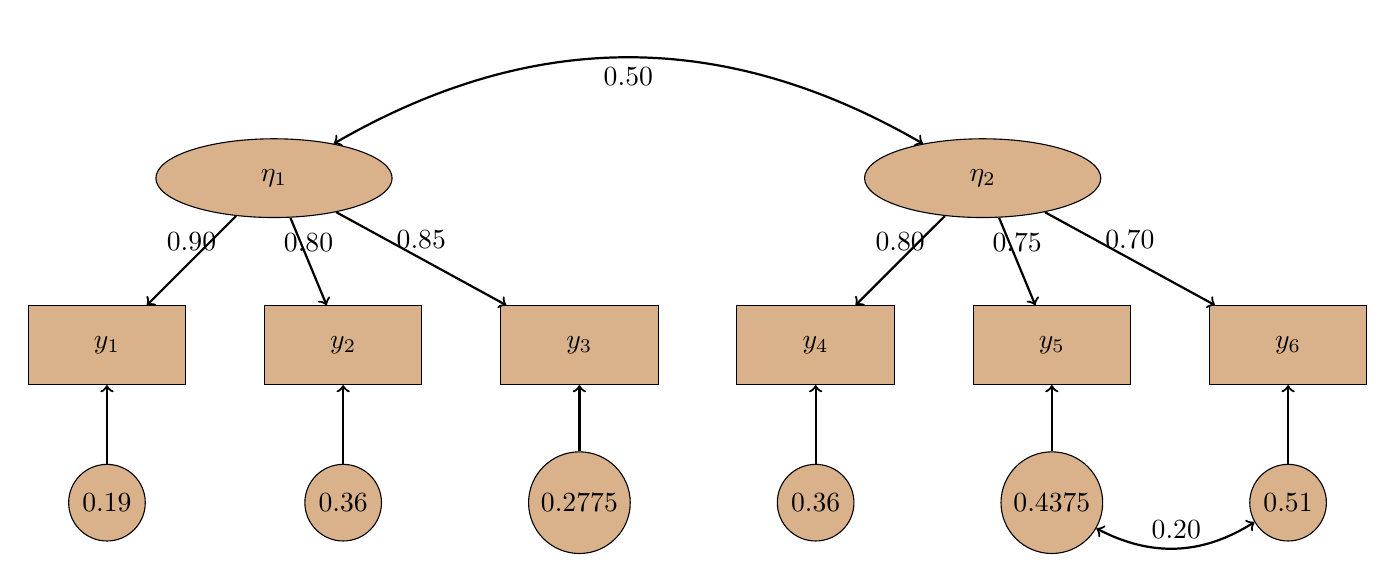
\begin{tikzpicture}[ factor/.style={draw,fill=brown!60, ellipse,minimum height=1cm, minimum width=3cm, node distance= {9cm}},
			latent/.style={draw,fill=brown!60, rectangle, minimum width=2cm, minimum height=1cm, node distance= {3cm}},
			residual/.style={draw,fill=brown!60,  circle, node distance= {2cm}}
			]
			\node [factor](x1) {$\eta_1$};
			\node [factor](x2)[right of =x1] {$\eta_2$};
			\node [latent](y1) [below left of=x1] {$y_1$};
			\node [latent](y2) [right of=y1] {$y_2$};
			\node [latent](y3) [right of=y2] {$y_3$};
			\node [latent](y4) [right of =y3] {$y_4$};
			\node [latent](y5) [right of=y4] {$y_5$};
			\node [latent](y6) [right of=y5] {$y_6$};
			\node [residual](e1) [below of=y1] {0.19};
			\node [residual](e2) [below of=y2] {0.36};
			\node [residual](e3) [below of=y3] {0.2775};
			\node [residual](e4) [below of=y4] {0.36};
			\node [residual](e5) [below of=y5] {0.4375};
			\node [residual](e6) [below of=y6] {0.51};
			
			\draw[thick, black, ->](x1) -- (y1) node[midway, above] {0.90};
			\draw[thick, black, ->] (x1) -- (y2) node[midway, above] {0.80};
			\draw[thick, black, ->] (x1) -- (y3) node[midway, above] {0.85};
			\draw[thick, black, ->] (x2) -- (y4) node[midway, above] {0.80};
			\draw[thick, black, ->] (x2) -- (y5) node[midway, above] {0.75};
			\draw[thick, black, ->] (x2) -- (y6) node[midway, above] {0.70};
			\draw[thick, black, ->] (e1) -- (y1);
			\draw[thick, black, ->] (e2) -- (y2);
			\draw[thick, black, ->] (e3) -- (y3);
			\draw[thick, black, ->] (e4) -- (y4);
			\draw[thick, black, ->] (e5) -- (y5);
			\draw[thick, black, ->] (e6) -- (y6);
			\draw[thick, black, <->] (e5) edge[bend right=30] node[above] {0.20} (e6);
			\draw[thick, black, <->] (x1) edge[bend left=30] node[below] {0.50} (x2);
		\end{tikzpicture}
	\end{adjustbox}
		\caption{Two factor CFA model with no error covariance}
		\label{fig:Figure 3.2}
	\end{figure}
\end{frame}
\begin{frame}
The predicted variance of $y_2$ is;\\
\begin{align*}
	Var(y_2)=\sigma_{22}=\lambda^2_{21} \psi_{11} +\theta_{12}\\
	=0.80^2(1)+0.36\\
	=1
\end{align*}
\end{frame}
\begin{frame}
The predicted(covariance) between $y_2$ and $y_3$ would be estimated as follows;
\begin{align*}
	Cov(y_2, y_3)=\lambda_{21} \psi_{11}\lambda_{31} +\theta_{23}\\
	=(0.80)1(0.85) +0\\
	=0.68
\end{align*}
\end{frame}
\begin{frame}
	And the predicted covariance (correlation) between $y_3$ and $y_4$ (Indicators that load on separate factors) would be estimated as follows:
	\begin{align*}
		Cov(y_3,y_4)=\sigma_{43}= \lambda_{31}\psi_{21}\lambda_{42}+\theta_{43}\\
		=(0.85)(0.5)(0.8)+0\\
		=0.34
	\end{align*}
\end{frame}
\begin{frame}
	This model also contains a correlation between the errors of the $y_5$ and $y_6$ indicators ($\theta_{65}$ =0.20). In this instance, the covariation between the indicators is not accounted for fully by the factor ($\eta_2$);$y_5$ and $y_6$ share additional variance owing to influences other than the latent construct and the predicted correlation between the two indicators is;
	\begin{align*}
		Cov(y_5,y_6)=\sigma_{56}=\lambda_{52}\psi_{22}\lambda_{62}+\theta_{65}\\
		=(0.75)\times1\times(0.70)+0.20\\
		=0.725
	\end{align*}
\end{frame}
\begin{frame}{Estimation of CFA Model Parameters}

The goal of latent variable measurement model is to establish the number and nature of factors that account for the variation and covariation among a set of indicators.The observed measures are intercorrelated because they are influenced by the same underlying constructs.If the latent constructs were partialed out the intercorrelations among observed measures would be zero.Thus CFA provides a more parsimonious understanding of the covariation among a set of indicators because the number of factors is less than the number of measured variables.\\

\noindent Factor analysis partitions the variance of each indicator(derived from the sample correlation or covariance matrix) into two parts: ‘common variance’, which is the variance which is estimated on the basis of the variance shared with other indicators in the analysis.and ‘unique variance’, which is a combination of reliable variance specific to the indicator and random error variance (measurement error or unreliability in the indicator).
\end{frame}
\begin{frame}
{Model Estimation}
All CFA models contain the parameters of factor loadings, unique variances and factor variances.If substantively justified, a CFA can include ‘error covariances’ which designate that two indicators  covary for reasons other than the shared influence of the latent factor eg (method effects).When CFA solution has two or more factors,a factor covariance is almost always specified to estimate the relationship between the latent dimensions.
\end{frame}
\begin{frame}
{Scaling The Latent}
Latent variables may either be exogenous(not caused by other variables in the model) or endogenous(caused by one or more variables in the model).Thus exogenous variables can be viewed as synonymous with X , independent or predictor variables.Similarly endogenous variables, dependent or outcome variables.\\
\noindent CFAs are considered to be exogenous variable models because the latent variables are specified to be freely intercorrelated without directional relationship among them.However,when CFA analysis includes covariates,as in MIMIC model (Brown 2006),or higher order factors,then the factors are endogenous.\\
\end{frame}
\begin{frame}
\noindent Latent variables have no inherent metrics; thus their units of measurements must be defined by the researcher.In CFA, this is accomplished in one of two ways.The most widely used method is the ‘Marker Indicator’ approach.This specification serves the function of passing the metric of the marker indicator along to the latent variable.In the second method, the variance of the latent variable is fixed to a value of 1.0.Although most CFA results are identical to the marker indicator approach when the factor variance is fixed to 1.0, this method does not produce an unstandardized solution.
\end{frame}
\begin{frame}
{Statistical Model Identification}
It is the concept that a CFA solution can be estimated only if the number of freely estimated parameters(eg factor loadings,uniqueness,factor correlations) does not exceed the number of pieces of information in the input matrix( number of sample variances and covariances).A model is overidentified when the number of knowns(individual elements of the input matrix) exceeds the number of unkowns(freely estimated parameters of the CFA solution)\\
The difference in the number of knowns and unknowns constitutes the model’s degrees of freedom(df).Overidentified solutions have a positive degrees of freedom.If the number of knowns equals the number of unknowns,the model has zero df and is said to be ‘just identified’.When the number of freely estimated parameters exceeds the number of pieces of information in the input matrix,the df is negative and the model is underidentified.\\
\end{frame}
\begin{frame}
An example of under-identified model input matrix is 
$$A=\begin{pmatrix}
	&Y_1  & Y_2\\ 
	Y_1& \sigma _{11} & \\ 
	Y_2& \sigma _{21}  & \sigma _{22} 
\end{pmatrix}$$
We have 3 elements of input matrix while the number of freely estimated model parameters is 4.( 2 factor loading and 2 error variances).The df=3-4=-1
\end{frame}
\begin{frame}{Illustration}
	\begin{figure}[h]
		\centering
		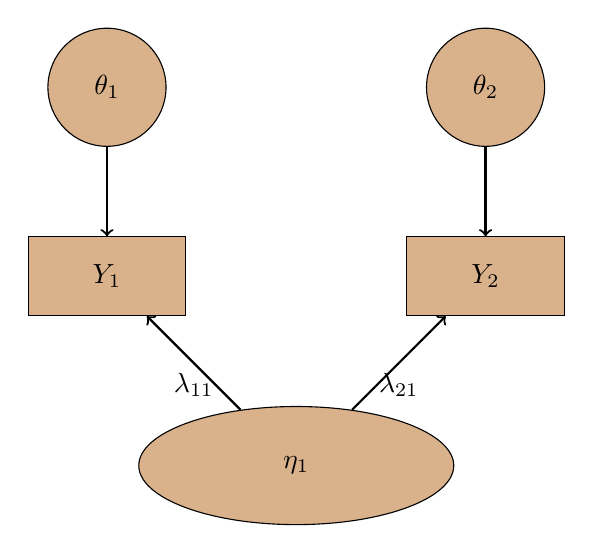
\begin{tikzpicture}[ factor/.style={draw,fill=brown!60, ellipse,minimum height=1.5cm, minimum width=4cm, node distance= {9cm}},
			latent/.style={draw, rectangle, minimum width=2cm, minimum height=1cm, fill=brown!60,node distance= {3.4cm}},
			residual/.style={draw,fill=brown!60,  circle, minimum width=1.5cm, minimum height=0.7cm, node distance= {2.4cm}}
			]
			\node [factor](x1) {$\eta_1$};
			\node [latent](y1) [above left of=x1] {$Y_1$};
			\node [latent](y2) [above right of=x1] {$Y_2$};
			\node [residual](e1) [above of=y1] {$\theta_1$};
			\node [residual](e2) [above of=y2] {$\theta_2$};
			\draw[thick, black, ->](x1) -- (y1) node[midway, below] {$\lambda_{11}$};
			\draw[thick, black, ->] (x1) -- (y2) node[midway, below] {$\lambda_{21}$};
			\draw[thick, black, ->] (e1) -- (y1);
			\draw[thick, black, ->] (e2) -- (y2);
		\end{tikzpicture}
		\label{Fig: Figure 3.2}
	\end{figure}
\end{frame}
\begin{frame}
	\noindent An example of just-identified model is:
	\begin{figure}[h]
		\centering
		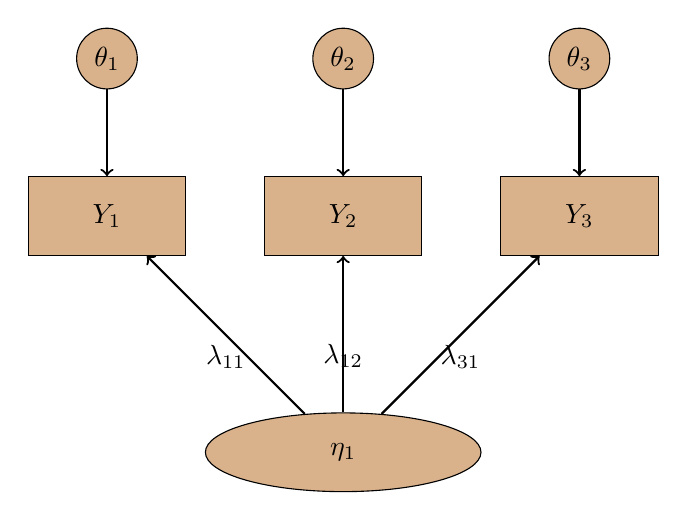
\begin{tikzpicture}[ factor/.style={draw,fill=brown!60, ellipse,minimum height=1cm, minimum width=3.5cm, node distance= {9cm}},
			latent/.style={draw, rectangle, minimum width=2cm, minimum height=1cm, fill=brown!60,node distance= {3cm}},
			residual/.style={draw,fill=brown!60,  circle, node distance= {2cm}}
			]
			\node [factor](x1) {$\eta_1$};
			
			\node [latent](y2) [above of=x1] {$Y_2$};
			\node [latent](y1) [left of=y2] {$Y_1$};
			
			\node [latent](y3) [right of =y2] {$Y_3$};
			
			\node [residual](e1) [above of=y1] {$\theta_1$};
			\node [residual](e2) [above of=y2] {$\theta_2$};
			
			\node [residual](e3) [above of=y3] {$\theta_3$};
			
			
			\draw[thick, black, ->](x1) -- (y1) node[midway, below] {$\lambda_{11}$};
			
			\draw[thick, black, ->] (x1) -- (y2) node[midway, below] {$\lambda_{12}$};
			
			\draw[thick, black, ->] (x1) -- (y3) node[midway, below] {$\lambda_{31}$};
			
			\draw[thick, black, ->] (e1) -- (y1);
			\draw[thick, black, ->] (e2) -- (y2);
			
			\draw[thick, black, ->] (e3) -- (y3);
			
		\end{tikzpicture}
		\label{Fig: Figure 3.3}
	\end{figure}
\end{frame}
\begin{frame}
	\noindent Input matrix is :
	
	$$B=\begin{pmatrix}
		& Y_1 & Y_2  & Y_3\\ 
		Y_1& \sigma_{11} &  & \\ 
		Y_2& \sigma_{21} & \sigma_{22} & \\ 
		Y_3&  \sigma_{31}&\sigma_{32}  & \sigma_{33}
	\end{pmatrix}$$
	We have 6 elements in the input matrix and 6 freely estimated model parameters.The df=6-6=0
\end{frame}
\begin{frame}{Overidentified model}
\begin{figure}[h]
	\centering
	\begin{adjustbox}{width=\textwidth}
	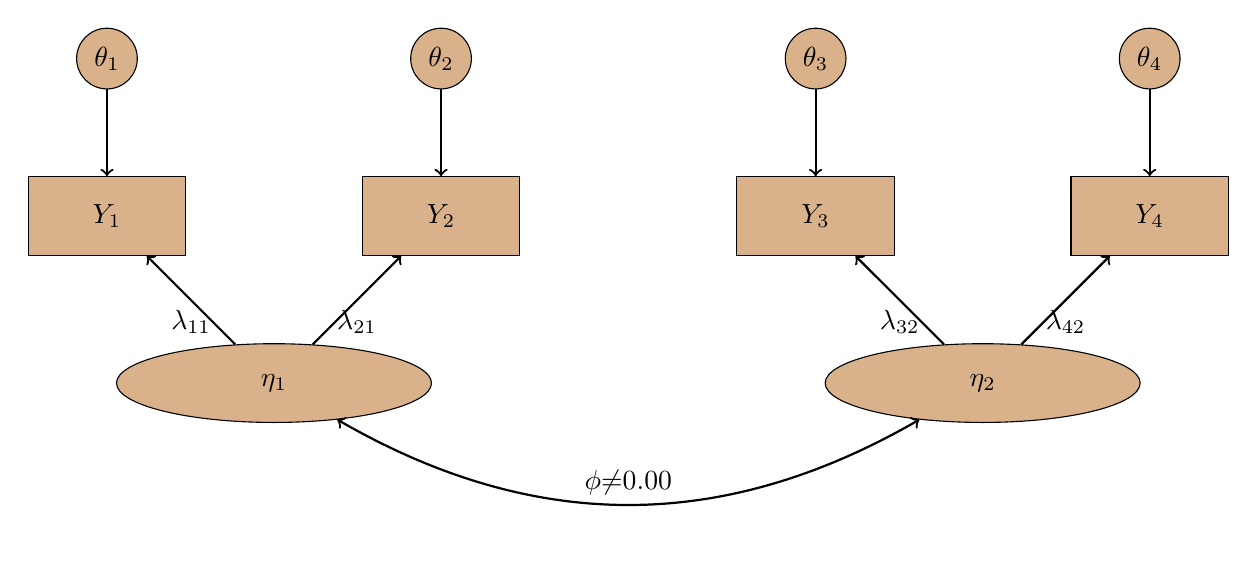
\begin{tikzpicture}[ factor/.style={draw,fill=brown!60, ellipse,minimum height=1cm, minimum width=4cm, node distance= {9cm}},
		latent/.style={draw, rectangle, minimum width=2cm, minimum height=1cm, fill=brown!60,node distance= {3cm}},
		residual/.style={draw,fill=brown!60,  circle, node distance= {2cm}}
		]
		\node [factor](x1) {$\eta_1$};
		\node [factor](x2)[right of =x1] {$\eta_2$};
		
		\node [latent](y1) [above left of=x1] {$Y_1$};
		\node [latent](y2) [above right of=x1] {$Y_2$};
		
		\node [latent](y3) [above left of =x2] {$Y_3$};
		\node [latent](y4) [above right of=x2] {$Y_4$};
		
		\node [residual](e1) [above of=y1] {$\theta_1$};
		\node [residual](e2) [above of=y2] {$\theta_2$};
		
		\node [residual](e3) [above of=y3] {$\theta_3$};
		\node [residual](e4) [above of=y4] {$\theta_4$};
		
		
		\draw[thick, black, ->](x1) -- (y1) node[midway, below] {$\lambda_{11}$};
		\draw[thick, black, ->] (x1) -- (y2) node[midway, below] {$\lambda_{21}$};
		
		\draw[thick, black, ->] (x2) -- (y3) node[midway, below] {$\lambda_{32}$};;
		\draw[thick, black, ->] (x2) -- (y4) node[midway, below] {$\lambda_{42}$};;
		
		\draw[thick, black, ->] (e1) -- (y1);
		\draw[thick, black, ->] (e2) -- (y2);
		
		\draw[thick, black, ->] (e3) -- (y3);
		\draw[thick, black, ->] (e4) -- (y4);
		
		\draw[thick, black, <->] (x1) edge[bend right=30] node[above] {$\phi$$\neq$0.00} (x2);
		
	\end{tikzpicture}
	\end{adjustbox}
	\label{fig:Figure 3.4}
\end{figure}
\end{frame}
\begin{frame}
	\noindent Input matrix is :\\
	
	$$C=\begin{pmatrix}
		& Y_1 & Y_2  & Y_3 & Y_4\\ 
		Y_1& \sigma_{11} &  & \\ 
		Y_2& \sigma_{21} & \sigma_{22} & \\ 
		Y_3&  \sigma_{31}&\sigma_{32}  & \sigma_{33} &\\
		Y_3&  \sigma_{31}&\sigma_{32}  & \sigma_{33} & \sigma_{44}
	\end{pmatrix}$$
	
	\noindent Note, df=10-9=1
\end{frame}
\begin{frame}
	Let b be the number of elements in the input matrix, and p be the number of indicators included in the input matrix, then\\
	$$b = p(p + 1)/2$$
\end{frame}
\begin{frame}
	{Descriptive Goodness Of Fit Indices}
	One of the several models that can be used to estimate CFA models is ML (Maximum Likelyhood).\\
	\noindent \textbf{\underline{Assumptions of ML}}
	
	\begin{enumerate}
		\item The sample size is large (n $\geq$ 200)
		\item The indicators of the factors have been measured on continuous scale
		\item The distribution of the indicators is multivariate normal.
	\end{enumerate}
\end{frame}
\begin{frame}
Although the actual parameter estimates may not be affected,non-normality in ML analysis can result in biased standard errors and goodness of -fit statistics.
If non-normality is extreme, then ML will produce incorrect parameter estimates thus incase of non-normal continuous indicators it is better to use a different estimator such as ML with robust standard errors and chi-square (Satorra and Bentler, 1994).
\end{frame}
\begin{frame}
There are a variety of goodness of fit statistics that provide a global desciptive summary of the ability of the model to reproduce the input covariance matrix. The classic goodness of fit is chi-square.
The idea is to test the hypothesis
$$H_0: S= \sum$$
$$H_1: S \neq \sum$$
The null hypothesis that the sample and model- implied variance – covariance matrices do not differ is retained.On the other hand a statistically significant chi square would lead to rejection of the null hypothesis meaning that the model estimates do not sufficiently reproduce the sample variances and covariances.
\end{frame}
\begin{frame}
\noindent \textbf{\underline{NOTE}}\\
Under typical ML model estimation ${\chi}^2$ is defined as 
$$ {\chi}^2 = F_{ML}{(n-1)}$$ 
Except in M-plus where ${\chi}^2 = F_{ML}(n)$
If $\alpha$ is chosen as a level of significance then the critical value for the test is ${\chi}^2_\alpha (df)$. Where df = the number of known values - number of free parameters.\\
We reject the null hypothesis that $S= \sum$ at $\alpha$ level of significance if ${\chi}^2 = (n-1) F_{ML} > {\chi}^2_{\alpha (df)}$ and conclude that the model estimate do not sufficiently reproduce the sample variance and covariances (i.e., the model is not a good fit to the data. Otherwise we do not reject the null hypothesis.\\
\end{frame}
\begin{frame}
	In conclusion the model ${\chi}^2$ is the meaningful test only when we have an overidentified model so that there is a degrees of freedom left over after accounting for all the three parameters in our model.\\
	The major drawback of chi square is that it is highly sensitive to sample size.
	While chi square is routinely reported in CFA research, there are other fit indices which are used in the evaluation of model fit.
\end{frame}
\begin{frame}
These are;
\begin{enumerate}
	\item \textbf{Root Mean Square Error of Approximationl}\\
	It is a population based index that relies on the noncentral chi square distribution, which is the distribution of the fitting function (e.g $F_{ML}$) when the fit of the model is not perfect.The model chi square and RMSEA belong to the class of indices called absolute fit indices.RMSEA is an error of approximation indexbecause it asseses the extent to which a model fit reasonably well in the population.
\end{frame}

\end{document}